\documentclass[a4paper]{article}
\usepackage[a4paper, margin=1in]{geometry}
% Some basic packages
\usepackage[utf8]{inputenc}
\usepackage[T1]{fontenc}
\usepackage{textcomp}
\usepackage[dutch]{babel}
\usepackage{url}
\usepackage{graphicx}
\usepackage{float}
\usepackage{booktabs}
\usepackage{enumitem}

\pdfminorversion=7

% Don't indent paragraphs, leave some space between them
\usepackage{parskip}

% Hide page number when page is empty
\usepackage{emptypage}
\usepackage{subcaption}
\usepackage{multicol}
\usepackage{xcolor}

% Other font I sometimes use.
% \usepackage{cmbright}

% Math stuff
\usepackage{amsmath, amsfonts, mathtools, amsthm, amssymb}
% Fancy script capitals
\usepackage{mathrsfs}
\usepackage{cancel}
% Bold math
\usepackage{bm}
% Some shortcuts
\newcommand\N{\ensuremath{\mathbb{N}}}
\newcommand\R{\ensuremath{\mathbb{R}}}
\newcommand\Z{\ensuremath{\mathbb{Z}}}
\renewcommand\O{\ensuremath{\emptyset}}
\newcommand\Q{\ensuremath{\mathbb{Q}}}
\newcommand\C{\ensuremath{\mathbb{C}}}

% Easily typeset systems of equations (French package)
\usepackage{systeme}

% Put x \to \infty below \lim
\let\svlim\lim\def\lim{\svlim\limits}

%Make implies and impliedby shorter
\let\implies\Rightarrow
\let\impliedby\Leftarrow
\let\iff\Leftrightarrow
\let\epsilon\varepsilon

% Add \contra symbol to denote contradiction
\usepackage{stmaryrd} % for \lightning
\newcommand\contra{\scalebox{1.5}{$\lightning$}}

% \let\phi\varphi

% Command for short corrections
% Usage: 1+1=\correct{3}{2}

\definecolor{correct}{HTML}{009900}
\newcommand\correct[2]{\ensuremath{\:}{\color{red}{#1}}\ensuremath{\to }{\color{correct}{#2}}\ensuremath{\:}}
\newcommand\green[1]{{\color{correct}{#1}}}

% horizontal rule
\newcommand\hr{
    \noindent\rule[0.5ex]{\linewidth}{0.5pt}
}

% hide parts
\newcommand\hide[1]{}

% si unitx
\usepackage{siunitx}
\sisetup{locale = FR}

% Environments
\makeatother
% For box around Definition, Theorem, \ldots
\usepackage{mdframed}
\mdfsetup{skipabove=1em,skipbelow=0em}
\theoremstyle{definition}
\newmdtheoremenv[nobreak=true]{definitie}{Definitie}
\newmdtheoremenv[nobreak=true]{eigenschap}{Eigenschap}
\newmdtheoremenv[nobreak=true]{gevolg}{Gevolg}
\newmdtheoremenv[nobreak=true]{lemma}{Lemma}
\newmdtheoremenv[nobreak=true]{propositie}{Propositie}
\newmdtheoremenv[nobreak=true]{stelling}{Stelling}
\newmdtheoremenv[nobreak=true]{wet}{Wet}
\newmdtheoremenv[nobreak=true]{postulaat}{Postulaat}
\newmdtheoremenv{conclusie}{Conclusie}
\newmdtheoremenv{toemaatje}{Toemaatje}
\newmdtheoremenv{vermoeden}{Vermoeden}
\newtheorem*{herhaling}{Herhaling}
\newtheorem*{intermezzo}{Intermezzo}
\newtheorem*{notatie}{Notatie}
\newtheorem*{observatie}{Observatie}
\newtheorem*{oef}{Oefening}
\newtheorem*{opmerking}{Opmerking}
\newtheorem*{praktisch}{Praktisch}
\newtheorem*{probleem}{Probleem}
\newtheorem*{terminologie}{Terminologie}
\newtheorem*{toepassing}{Toepassing}
\newtheorem*{uovt}{UOVT}
\newtheorem*{vb}{Voorbeeld}
\newtheorem*{vraag}{Vraag}

\newmdtheoremenv[nobreak=true]{definition}{Definition}
\newtheorem*{eg}{Example}
\newtheorem*{notation}{Notation}
\newtheorem*{previouslyseen}{As previously seen}
\newtheorem*{remark}{Remark}
\newtheorem*{note}{Note}
\newtheorem*{problem}{Problem}
\newtheorem*{observe}{Observe}
\newtheorem*{property}{Property}
\newtheorem*{intuition}{Intuition}
\newmdtheoremenv[nobreak=true]{prop}{Proposition}
\newmdtheoremenv[nobreak=true]{theorem}{Theorem}
\newmdtheoremenv[nobreak=true]{corollary}{Corollary}

% End example and intermezzo environments with a small diamond (just like proof
% environments end with a small square)
\usepackage{etoolbox}
\AtEndEnvironment{vb}{\null\hfill$\diamond$}%
\AtEndEnvironment{intermezzo}{\null\hfill$\diamond$}%
% \AtEndEnvironment{opmerking}{\null\hfill$\diamond$}%

% Fix some spacing
% http://tex.stackexchange.com/questions/22119/how-can-i-change-the-spacing-before-theorems-with-amsthm
\makeatletter
\def\thm@space@setup{%
  \thm@preskip=\parskip \thm@postskip=0pt
}


% Exercise 
% Usage:
% \oefening{5}
% \suboefening{1}
% \suboefening{2}
% \suboefening{3}
% gives
% Oefening 5
%   Oefening 5.1
%   Oefening 5.2
%   Oefening 5.3
\newcommand{\oefening}[1]{%
    \def\@oefening{#1}%
    \subsection*{Oefening #1}
}

\newcommand{\suboefening}[1]{%
    \subsubsection*{Oefening \@oefening.#1}
}


% \lecture starts a new lecture (les in dutch)
%
% Usage:
% \lecture{1}{di 12 feb 2019 16:00}{Inleiding}
%
% This adds a section heading with the number / title of the lecture and a
% margin paragraph with the date.

% I use \dateparts here to hide the year (2019). This way, I can easily parse
% the date of each lecture unambiguously while still having a human-friendly
% short format printed to the pdf.

\usepackage{xifthen}
\def\testdateparts#1{\dateparts#1\relax}
\def\dateparts#1 #2 #3 #4 #5\relax{
    \marginpar{\small\textsf{\mbox{#1 #2 #3 #5}}}
}

\def\@lecture{}%
\newcommand{\lecture}[3]{
    \ifthenelse{\isempty{#3}}{%
        \def\@lecture{Lecture #1}%
    }{%
        \def\@lecture{Lecture #1: #3}%
    }%
    \subsection*{\@lecture}
    \marginpar{\small\textsf{\mbox{#2}}}
}



% These are the fancy headers
\usepackage{fancyhdr}
\pagestyle{fancy}

% LE: left even
% RO: right odd
% CE, CO: center even, center odd
% My name for when I print my lecture notes to use for an open book exam.
% \fancyhead[LE,RO]{Gilles Castel}

\fancyhead[RO,LE]{\@lecture} % Right odd,  Left even
\fancyhead[RE,LO]{}          % Right even, Left odd

\fancyfoot[RO,LE]{\thepage}  % Right odd,  Left even
\fancyfoot[RE,LO]{}          % Right even, Left odd
\fancyfoot[C]{\leftmark}     % Center

\makeatother




% Todonotes and inline notes in fancy boxes
\usepackage{todonotes}
\usepackage{tcolorbox}

% Make boxes breakable
\tcbuselibrary{breakable}

% Verbetering is correction in Dutch
% Usage: 
% \begin{verbetering}
%     Lorem ipsum dolor sit amet, consetetur sadipscing elitr, sed diam nonumy eirmod
%     tempor invidunt ut labore et dolore magna aliquyam erat, sed diam voluptua. At
%     vero eos et accusam et justo duo dolores et ea rebum. Stet clita kasd gubergren,
%     no sea takimata sanctus est Lorem ipsum dolor sit amet.
% \end{verbetering}
\newenvironment{verbetering}{\begin{tcolorbox}[
    arc=0mm,
    colback=white,
    colframe=green!60!black,
    title=Opmerking,
    fonttitle=\sffamily,
    breakable
]}{\end{tcolorbox}}

% Noot is note in Dutch. Same as 'verbetering' but color of box is different
\newenvironment{noot}[1]{\begin{tcolorbox}[
    arc=0mm,
    colback=white,
    colframe=white!60!black,
    title=#1,
    fonttitle=\sffamily,
    breakable
]}{\end{tcolorbox}}




% Figure support as explained in my blog post.
\usepackage{import}
\usepackage{xifthen}
\usepackage{pdfpages}
\usepackage{transparent}
\newcommand{\incfig}[1]{%
    \def\svgwidth{\columnwidth}
    \import{./figures/}{#1.pdf_tex}
}

% Fix some stuff
% %http://tex.stackexchange.com/questions/76273/multiple-pdfs-with-page-group-included-in-a-single-page-warning
\pdfsuppresswarningpagegroup=1

\title{\Huge{Machine Learning and Statistical Theory II}\\ Generalized Linear Models}
\author{\huge{Daniel Yu}}
\date{September 18,2024}

\pdfsuppresswarningpagegroup=1

\begin{document}
\maketitle
\newpage% or \cleardoublepage
% \pdfbookmark[<level>]{<title>}{<dest>}
\tableofcontents
\pagebreak
\section{Generalized Linear Models}
Note: Generalized Linear Models and Splines can be grouped and used together

\subsection{Regression}
Recall 2 forms of regression:
\begin{enumerate}
  \item Linear Regression: ($y \in \R$) $Y = \vec{B}^T \vec{X} + \epsilon$ where  $\epsilon \sim Normal\left( 0, \sigma^2 \right) $
  \item Logistic Regresion:($y \in \{0,1\} $) $\log \frac{P(Y=1 | X)}{1-P(Y=1| X)} = \vec{B}^T \vec{X}$
\end{enumerate}

\begin{definition}
  A \textbf{transformation (link} is defined as follows. There exists a $g(u)$, the link, where $u = E(Y | \vec{X})$ such that
  while the expected value may not be linear, some function of it is linear, i.e.:
   \[
     g(E[Y| \vec{X}]) = g(\vec{X}) = \vec{B}^T X 
  .\] 
  We need the link function to be invertible
\end{definition}

\begin{remark}
  This can be thought of as analogous to having \textbf{basis} elements which could be anything but still form a 
  vector space where the outputs are linear in regards to these potentially non-linear basis elements. 
  For example, consider the vector space of polynomials of degree $n$. 
\end{remark}

\begin{note}{Example} \\
  linear regression
  \[
  g(u) = I \cdot u = u
  .\] 
  logistic regression:
  \[
    g(u) = \log(\frac{u}{1-u}) = \vec{B}^T X 
  .\] 
  The above is a linear equation in terms of $B_i, X_i$, even though \textbf{probability p and X are nonlinear} 
\end{note}

\begin{note}
  GLM can be viewed as addressing different distributions
  \begin{enumerate}
    \item linear regression - Assume $Y | \vec{X} \sim Normal(\mu=\vec{B}^T X, \sigma^2)$ 
    \item logistic regression - Assume $Y | \vec{X} \sim Ber(p)$
    \item Poission ???
  \end{enumerate}
\end{note}

\begin{definition}{Generalized Linear Models} \\
GLM is a flexible extension of ordinary linear regression that allows for response variables (dependent variables) 
that have error distribution models other than a normal distribution. GLMs consist of three components:  
\begin{enumerate}
  \item Random Component: $Y | X \sim $ some distribution. (In practice, GLM work particularly well with exponential family of 
    distributions
  \item Linear Assumption: Assume there is a linear predictor $\vec{\xi} = \vec{B}^T X$
  \item Link: Between random and covariates  $\vec{X}$:
    \[
  g(u(\vec{X})) = g(E(Y | \vec{X})) = \vec{\xi} = \vec{B}^T X 
    .\] and we want $g$ to be invertible
\end{enumerate}
\end{definition}

\begin{note}{Exponential Family} \\
  The exponential family of distributions (works best for GLM):
  \begin{enumerate}
    \item Gaussian
    \item Bernoulli
    \item Binomial 
    \item Multinomial 
    \item Possion
    \item Exponential
    \item Gamma
    \item Laplace
    \item Beta
    \item etc.
  \end{enumerate}
  Stuff like \textbf{student t, mixture, some uniform distributions} are not exponential
\end{note}

\section{Exponential Family}
\begin{definition}
  A pdf of a distribution in d-params with the following form is a d-param exponential family density:
  \begin{align*}
     p(\vec{y}; \vec{n}) &= \frac{1}{Z(\vec{n})} h(\vec{y}) \exp [\vec{n} T(\vec{y})] \\
                        &= h(\vec{y}) \exp [\vec{n} T(y) - A(\vec{n})] 
  .\end{align*}
      where $A(\vec{n}) = \log Z(\vec{n})$
  \begin{enumerate}
    \item $\vec{n} \in \R^d$ is a natural param of distribution
    \item $T(\vec{y}) \in \R^d$ is vector of sufficient statistics (usually $T(\vec{y}) = \vec{y}$). 
      For example, for normal this would be a vector of sample mean and variance
    \item $h(\vec{y})$ is underlying measure (usually $h(\vec{y}) = 1$) 
    \item $A(\vec{n}) = \log Z(\vec{n})$ is the log normalizer, exists to make sure integral of pdf = 1
      \[
        A(\vec{n}) = \log \int h(y) \exp(\vec{n}^T T(\vec{y})) dy
      .\] 
  \end{enumerate}
\end{definition}
\begin{figure}[h]
  \centering
  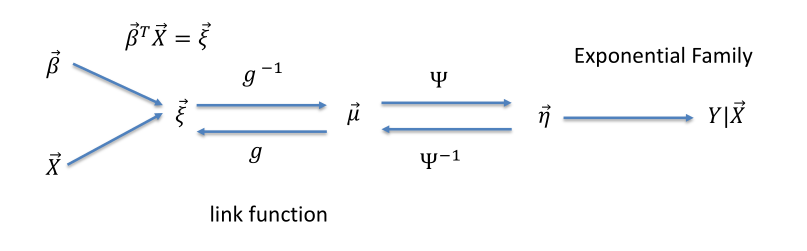
\includegraphics[width=0.8\textwidth]{assets/link_and_exponential.png}
  \caption{Relationship between Link and Exponential Family Distribution}
  \label{fig:link_and_exponential}
\end{figure}
Note that $\vec{u} = E(Y | X =\vec{x})$. Usually we assume $\xi = \vec{n}$ and  $g = \phi$, the \textbf{canonical link function},
in this case both sides become symmetric. Note that in this class we will be working with canonical link case. For 
canonical link:
\begin{enumerate}
  \item Normal: $g(\mu) = \mu$
  \item Binomial:  $g(\mu) = \log \frac{\mu}{1-\mu}$ (binary classification)
  \item poisson: $g(\mu) = \log(\mu)$
  \item gamma: $g(\mu) = - \frac{1}{\mu}$ 
  \item negative binomial: $g(\mu) = \log[\frac{\mu}{k(1+\frac{\mu}{k}}]$
\end{enumerate}

\begin{note}{Example - Bernoulli} \\
  Normal pdf: $p(y:u) = Ber(y:\mu) = \mu^y (1-\mu)^{1-y}$ where  $y \in \{0,1\} $ 
  \begin{align*}
    p(y:u) &= \mu^y (1-\mu)^{1-y} \\
           &= \exp(y \log(\mu) + (1-y) \log(1-\mu)) \\
           &= \exp(y \log(\frac{\mu}{1 - \mu}) + \log(1-\mu))
  .\end{align*}
  where $T(y) = y$,  $h(\vec{y}) = 1$,  $n=\log(\frac{\mu}{1-\mu})$, and $A(\vec{n}) = - \log(1-\mu)$. 

  Notice that this gives the link function $\mu = \frac{1}{1+e^{-n}}$ 
\end{note}


TODO Binomial


\end{document}
